\documentclass[mstat,12pt]{unswthesis}



%%%%%%%%%%%%%%%%%%%%%%%%%%%%%%%%%%%%%%%%%%%%%%%%%%%%%%%%%%%%%%%%%%
% 
% OK...Now we get to some actual input.  The first part sets up
% the title etc that will appear on the front page
%
%%%%%%%%%%%%%%%%%%%%%%%%%%%%%%%%%%%%%%%%%%%%%%%%%%%%%%%%%%%%%%%%%

\title{Capstone Project by Team D\\[0.5cm]A Data Science Approach to
Forecasting Electricity Demand in NSW, Australia}

\authornameonly{Baheerathan Gnanasundram, Matthew Seery, Mohammad Ahsan
Ullah, Rahul Lobo. }

\author{\Authornameonly}

\copyrightfalse
\figurespagefalse
\tablespagefalse

%%%%%%%%%%%%%%%%%%%%%%%%%%%%%%%%%%%%%%%%%%%%%%%%%%%%%%%%%%%%%%%%%
%
%  And now the document begins
%  The \beforepreface and \afterpreface commands puts the
%  contents page etc in
%
%%%%%%%%%%%%%%%%%%%%%%%%%%%%%%%%%%%%%%%%%%%%%%%%%%%%%%%%%%%%%%%%%%


%%%%%%%%%%%%%%%%%%%%%%%%%%%%%%%%%%%%%%%%%%%%%%%%%%%%%%%%%%%%%%%%%%%%%%%
%
%  A small sample UNSW Coursework Masters thesis file.
%  Any questions to Ian Doust i.doust@unsw.edu.au and/or Gery Geenens ggeenens@unsw.edu.au
%
%%%%%%%%%%%%%%%%%%%%%%%%%%%%%%%%%%%%%%%%%%%%%%%%%%%%%%%%%%%%%%%%%%%%%%%
%
%  The first part pulls in a UNSW Thesis class file.  This one is
%  slightly nonstandard and has been set up to do a couple of
%  things automatically
%
 
%%%%%%%%%%%%%%%%%
%% Precisely one of the next four lines should be uncommented.
%% Choose the one which matches your degree, uncomment it, and comment out the other two!
%\documentclass[mfin,12pt]{unswthesis}    %%  For Master of Financial Mathematics 
%\documentclass[mmath,12pt]{unswthesis}   %%  For Master of Mathematics
%\documentclass[mstat,12pt]{unswthesis}  %%  For Master of Statistics
%%%%%%%%%%%%%%%%%



\linespread{1}
\usepackage{amsfonts}
\usepackage{amssymb}
\usepackage{amsthm}
\usepackage{latexsym,amsmath}
\usepackage{graphicx}
\usepackage{afterpage}
\usepackage[colorlinks]{hyperref}
 \hypersetup{
     colorlinks=true,
     linkcolor=blue,
     filecolor=blue,
     citecolor= black,      
     urlcolor=cyan,
     }
\usepackage{textcomp}
\usepackage{longtable}
\usepackage{booktabs}
\usepackage{float}

%%%%%%%%%%%%%%%%%%%%%%%%%%%%%%%%%%%%%%%%%%%%%%%%%%%%%%%%%%%%%%%%%
%
%  The following are some simple LaTeX macros to give some
%  commonly used letters in funny fonts. You may need more or less of
%  these
%
\newcommand{\R}{\mathbb{R}}
\newcommand{\Q}{\mathbb{Q}}
\newcommand{\C}{\mathbb{C}}
\newcommand{\N}{\mathbb{N}}
\newcommand{\F}{\mathbb{F}}
\newcommand{\PP}{\mathbb{P}}
\newcommand{\T}{\mathbb{T}}
\newcommand{\Z}{\mathbb{Z}}
\newcommand{\B}{\mathfrak{B}}
\newcommand{\BB}{\mathcal{B}}
\newcommand{\M}{\mathfrak{M}}
\newcommand{\X}{\mathfrak{X}}
\newcommand{\Y}{\mathfrak{Y}}
\newcommand{\CC}{\mathcal{C}}
\newcommand{\E}{\mathbb{E}}
\newcommand{\cP}{\mathcal{P}}
\newcommand{\cS}{\mathcal{S}}
\newcommand{\A}{\mathcal{A}}
\newcommand{\ZZ}{\mathcal{Z}}
%%%%%%%%%%%%%%%%%%%%%%%%%%%%%%%%%%%%%%%%%%%%%%%%%%%%%%%%%%%%%%%%%%%%%
%
% The following are much more esoteric commands that I have left in
% so that this file still processes. Use or delete as you see fit
%
\newcommand{\bv}[1]{\mbox{BV($#1$)}}
\newcommand{\comb}[2]{\left(\!\!\!\begin{array}{c}#1\\#2\end{array}\!\!\!\right)
}
\newcommand{\Lat}{{\rm Lat}}
\newcommand{\var}{\mathop{\rm var}}
\newcommand{\Pt}{{\mathcal P}}
\def\tr(#1){{\rm trace}(#1)}
\def\Exp(#1){{\mathbb E}(#1)}
\def\Exps(#1){{\mathbb E}\sparen(#1)}
\newcommand{\floor}[1]{\left\lfloor #1 \right\rfloor}
\newcommand{\ceil}[1]{\left\lceil #1 \right\rceil}
\newcommand{\hatt}[1]{\widehat #1}
\newcommand{\modeq}[3]{#1 \equiv #2 \,(\text{mod}\, #3)}
\newcommand{\rmod}{\,\mathrm{mod}\,}
\newcommand{\p}{\hphantom{+}}
\newcommand{\vect}[1]{\mbox{\boldmath $ #1 $}}
\newcommand{\reff}[2]{\ref{#1}.\ref{#2}}
\newcommand{\psum}[2]{\sum_{#1}^{#2}\!\!\!'\,\,}
\newcommand{\bin}[2]{\left( \begin{array}{@{}c@{}}
				#1 \\ #2
			\end{array}\right)	}
%
%  Macros - some of these are in plain TeX (gasp!)
%
\newcommand{\be}{($\beta$)}
\newcommand{\eqp}{\mathrel{{=}_p}}
\newcommand{\ltp}{\mathrel{{\prec}_p}}
\newcommand{\lep}{\mathrel{{\preceq}_p}}
\def\brack#1{\left \{ #1 \right \}}
\def\bul{$\bullet$\ }
\def\cl{{\rm cl}}
\let\del=\partial
\def\enditem{\par\smallskip\noindent}
\def\implies{\Rightarrow}
\def\inpr#1,#2{\t \hbox{\langle #1 , #2 \rangle} \t}
\def\ip<#1,#2>{\langle #1,#2 \rangle}
\def\lp{\ell^p}
\def\maxb#1{\max \brack{#1}}
\def\minb#1{\min \brack{#1}}
\def\mod#1{\left \vert #1 \right \vert}
\def\norm#1{\left \Vert #1 \right \Vert}
\def\paren(#1){\left( #1 \right)}
\def\qed{\hfill \hbox{$\Box$} \smallskip}
\def\sbrack#1{\Bigl \{ #1 \Bigr \} }
\def\ssbrack#1{ \{ #1 \} }
\def\smod#1{\Bigl \vert #1 \Bigr \vert}
\def\smmod#1{\bigl \vert #1 \bigr \vert}
\def\ssmod#1{\vert #1 \vert}
\def\sspmod#1{\vert\, #1 \, \vert}
\def\snorm#1{\Bigl \Vert #1 \Bigr \Vert}
\def\ssnorm#1{\Vert #1 \Vert}
\def\sparen(#1){\Bigl ( #1 \Bigr )}

\newcommand\blankpage{%
    \null
    \thispagestyle{empty}%
    \addtocounter{page}{-1}%
    \newpage}

%%%%%%%%%%%%%%%%%%%%%%%%%%%%%%%
%
% These environments allow you to get nice numbered headings
%  for your Theorems, Definitions etc.  
%
%  Environments
%
%%%%%%%%%%%%%%%%%%%%%%%%%%%%%%%

\newtheorem{theorem}{Theorem}[section]
\newtheorem{lemma}[theorem]{Lemma}
\newtheorem{proposition}[theorem]{Proposition}
\newtheorem{corollary}[theorem]{Corollary}
\newtheorem{conjecture}[theorem]{Conjecture}
\newtheorem{definition}[theorem]{Definition}
\newtheorem{example}[theorem]{Example}
\newtheorem{remark}[theorem]{Remark}
\newtheorem{question}[theorem]{Question}
\newtheorem{notation}[theorem]{Notation}
\numberwithin{equation}{section}

%%%%%%%%%%%%%%%%%%%%%%%%%%%%%%%%%%%%%%%%%%%%%%%%%%%%%%%%%%%%%%%%%%
%
%  If you've got some funny special words that LaTeX might not
% hyphenate properly, you can give it a helping hand:
%

\hyphenation{Mar-cin-kie-wicz Rade-macher}






\begin{document}

\beforepreface

%\afterpage{\blankpage}

% plagiarism

\prefacesection{Plagiarism statement}

\vskip 2pc \noindent I declare that this thesis is my
own work, except where acknowledged, and has not been submitted for
academic credit elsewhere. 

\vskip 2pc  \noindent I acknowledge that the assessor of this
thesis may, for the purpose of assessing it:
\begin{itemize}
\item Reproduce it and provide a copy to another member of the University; and/or,
\item Communicate a copy of it to a plagiarism checking service (which may then retain a copy of it on its database for the purpose of future plagiarism checking).
\end{itemize}

\vskip 2pc \noindent I certify that I have read and understood the University Rules in
respect of Student Academic Misconduct, and am aware of any potential plagiarism penalties which may 
apply.\vspace{24pt}

\vskip 2pc \noindent By signing 
this declaration I am
agreeing to the statements and conditions above.
\vskip 2pc \noindent
Signed: \rule{7cm}{0.25pt} \hfill Date: \rule{4cm}{0.25pt} \\[1cm]
Signed: \rule{7cm}{0.25pt} \hfill Date: \rule{4cm}{0.25pt} \\[1cm]
Signed: \rule{7cm}{0.25pt} \hfill Date: \rule{4cm}{0.25pt} \\[1cm]
Signed: \rule{7cm}{0.25pt} \hfill Date: \rule{4cm}{0.25pt} \\[1cm]
\vskip 1pc

%\afterpage{\blankpage}

% Acknowledgements are optional


\prefacesection{Acknowledgements}

{\bigskip}All thanks must go to our families and university professors
who have guided us through this Capstone Project. Without them this
would not be possible.\\[1cm] 

{\bigskip\bigskip\bigskip\noindent} 15/06/2021.

%\afterpage{\blankpage}

% Abstract

\prefacesection{Abstract}

Forecasting electricity demand is an important requirement as there are
now more interested stakeholders associated with the generation and
distribution of this service. Traditionally electricity demand was just
the concern of governments. However, this has now been extended to
market bodies and owners and operators of the underlying infrastructure
required for this service. Forecasting accurate energy demand not only
supports network infrastructure, but also aides investment decisions
about power generation. It is thus of interest to a variety of
stakeholders including power utilities, energy policymakers, and private
investors just to name a few. This study aims to demonstrate how neural
network (specifically LSTM neural networks) can be used to accurately
forecast short-term energy demand. The focus will be on attributes such
as temperature, month of the year, day of the week and time of the day
as well as how past time lags can be used to predict future demand
values. It is envisaged that the results of this study will provide
useful insights for governments and market bodies to assist in the
rules, policies and pricing that are invoked on the energy sector.
Additionally, the businesses operating in this sector can use this
information to guide their decision-making regarding electricity
generation and distribution, as well as for the purpose of price
benchmarking.

%\afterpage{\blankpage}


\afterpreface





%%%%%%%%%%%%%%%%%%%%%%%%%%%%%%%%%%%%%%%%%%%%%%%%%%%%%%%%%%%%%%%%%%
%
% Now we can start on the first chapter
% Within chapters we have sections, subsections and so forth
%
%%%%%%%%%%%%%%%%%%%%%%%%%%%%%%%%%%%%%%%%%%%%%%%%%%%%%%%%%%%%%%%%%%



%%%%%%%%%%%%%%%%%%%%%%%%%%%%%%%%%%%%%

%\afterpage{\blankpage}


\hypertarget{introduction}{%
\chapter{Introduction}\label{introduction}}

Towards the end of the 20th century, countries throughout the world
began moving away from regulated government-controlled energy supply to
a deregulated sector influenced by market forces \cite{Catalao2007}.
This means that forecasting for electricity demands is essential
information required beyond previously regulated governmental
structures. It is now required by the market bodies working in the
sector and private industries who invest in the generation and
distribution of electricity. In turn, this aids in better rules,
policies, and pricing in the energy sector. However, for this study, the
focus will primarily be on short-term forecasting as this can greatly
aid vested parties concerned in maximising profits and cutting costs.

\bigskip

Temperature plays a significant role in electricity demand. This is
because heating is utilised more by customers in the cooler months while
cooling is required for the hottest months of the year. For that reason,
temperature is an essential attribute that will be investigated in this
study. However, temperature does not account for other factors such as
humidity or varying electricity usage patterns associated with specific
days of the weeks. For example, a temperature of 25 degrees in Spring
may not lead to as much usage of air conditioning as a humid day in
Summer with the same temperature. Additionally, the usage rate of
electricity will inevitably vary between weekdays, weekends, and public
holidays due to the varying ratios of usage between business and
residential customers. Therefore, the month of the year, day of the week
and time of day will also be examined in this study.

\hypertarget{literature-review}{%
\chapter{Literature Review}\label{literature-review}}

There have been various studies undertaken where more traditional
statistical methods such as multiple linear regression (MLR) have been
utilised to predict demand \cite{Mohamed2005}. However, in more recent
times there has been greater focus on the use of neural networks to help
solve the problem of forecasting demand \cite{Gonzalez2008}. The
advantage of neural networks is they are very suitable for determining
non-linear relationships \cite{Gonzalez2008} and have been widely used
for short-term demand forecasting \cite{Ciulla2019}. They are also very
flexible and easy to configure when dealing with time-series data
\cite{Carmona2002}. For neural networks, monthly values have been a
popular unit of measure and this is particularly true when short-term
forecasting of demand has been employed \cite{Carmona2002}. However,
this proposed solution differs because the focus will be on intervals
shorter than even a day as this is of greater interest to the client.
Nevertheless, the month of the year will still be considered as an input
factor for the model for its potential to distinguish factors such as
humidity that are not fully explained by temperature alone. Another
distinguishing factor for this study will be the emphasis on the day of
the week where each record will be categorised as either a weekday,
weekend, or public holiday.

\bigskip

Up until the time of writing, the majority of deep learning models being
appliied to energy forecasting fall under the subset of three major
types \cite{Kumar2013}. These are: A feed forward neural network
(FFNN)/Multi Layer Perceptron (MLP) through the process of increasing
the number of hidden layers, some form of recurrence through a recurrent
neural network (RNN), long-short term memory (LSTM) or gated recurrent
unit (GRU), or through sequentially combining different types of
algorithms into an overall structure. In 2020, Xue et al.~contrasted
these different approaches in order to forecast the heating demand of a
district system \cite{Xue2020}. Their experiments showed that the LSTM
models were amongst the highest-performing of the models tested.

\bigskip

When applied to natural gas forecasting, a close relative to electricity
demand, RNN models have proven to be useful in prediction. Wei et
al.~(2019) explored the application of LSTM for forecasting natural gas
consumption of four cities \cite{Xue2020}. In addition, LSTM models used
for forecasting were compared with other model techniques, including
multiple linear regression, feed-forward neural networks, and a support
vector regression in this study. The authors' rigorous testing
demonstrated that LSTM models achieved a greater accuracy than the other
data-driven models. It appears that RNN and LSTM models have formed the
majority of accurate forecasting implementations to date, with other
machine learning techniques such as SVMs performing as well as, but not
better than RNN and LSTM based models. An example of this is
demonstrated by Amarasignhe et al.~(2017), who contrasted the deep
learning techniques of a Convolutional Neural Network (CNN) and LSTM,
against a traditional machine learning technique (SVM) in order to
forecast the energy demand of a building. This forecast was for a time
period of sixty hours ahead and used 4 years of training data
\cite{Amarasinghe2016}. Their experiments proved that the deep learning
based forecasting models obtained less forecasting error when compared
with standard machine learning-based techniques; in particular, the LSTM
obtained the smallest error.

\bigskip

Due to the significance of the LSTM accuracy across a variety of these
studies, it will form the basis of this analysis.

\hypertarget{material-and-methods}{%
\chapter{Material and Methods}\label{material-and-methods}}

\hypertarget{software}{%
\section{Software}\label{software}}

A variety of software was used in the analysis as well as for
collaboration and organisational purposes. GitHub was used as the main
tool for collaboration and version control. It is not only extensively
used in the industry but also enables the ability to collaborate on code
seamlessly from local machines. This was the best choice as it is also
used in the course instruction.

\bigskip

For data analysis purposes, Python, R/Rstudio and Tableau were all used.
R was utilised in the initial exploratory data analysis phase in
conjunction with Tableau, to visualise the dataset and to observe any
obvious trends in the energy data. Tableau was especially useful in
visualisation as it allowed the segmentation of days, times and months
to be easily discerned in reference to energy demand. The main software
used for the electricity demand modelling was Python. It was also used
to clean, transform, and replace missing values in the supplied data and
for merging separate datasets including the final LSTM model which was
constructed.

\bigskip

Furthermore, Excel was used to fill in missing values for the
temperature dataset and the report for this analysis has been
constructed in RMarkdown.

\hypertarget{description-of-the-data}{%
\section{Description of the Data}\label{description-of-the-data}}

Three csv files were supplied for this project. The file
totaldemand\_nsw.csv contains three columns which record a date and
timestamp (DATETIME) for the electricity consumed (TOTALDEMAND) for the
associated region (REGIONID). The DATETIME columns contains dates
between the 1st of January 2010 and midnight on the 18th of March 2021.
Also included with each date is a timestamp with values for hours and
minutes. There is a timestamp for each hour and thirty-minute interval
within each hour for the aforementioned range of dates. All observations
have the same value for the REGIONID column which is `NSW1'.

\bigskip

The file temperature\_nsw.csv also contains three columns. The columns
record the location for the temperature observation (LOCATION), the date
and time it was recorded (DATETIME) and the actual recorded temperature
(TEMPERATURE). The values in the LOCATION column are all the same
containing the value `Bankstown' that describes the Bankstown weather
station. The values in the DATETIME column are in the same format and
range of dates as the temperature\_nsw.csv file except some observations
are outside the on hour or thirty-minute interval within each hour time
periods. The file also contains duplicates and has missing values
between the dates of the 1st of January 2010 and 18th of March 2021.

\bigskip

The third file, forecastdemand\_nsw.csv, contains periodic forecasts
(FORECASTDEMAND) for a set date and time (DATETIME) and the date and
time the forecast was made (LASTCHANGED). The values in the
FORECASTDEMAND column align with the same range of dates in the
totaldemand\_nsw.csv file. The format of the date and time in this
column and the DATETIME column is the same as the DATETIME column in the
totaldemand\_nsw.csv file. The forecastdemand\_nsw.csv file also
includes a REGIONID column and all with the same values as the
totaldemand\_nsw.csv file. There is also a column called
PREDISPATCHSEQNO which contains a unique id number for each forecast and
a PERIODID column which contains a unique ID for forecasts of each
unique date and time in the DATETIME column. The data in this file was
not used in the neural network models that were tested.

\hypertarget{pre-processing-steps-and-data-cleaning}{%
\section{Pre-processing Steps and Data
Cleaning}\label{pre-processing-steps-and-data-cleaning}}

The data in the file totaldemand\_nsw.csv required no further cleaning
other than the removal of the REGIONID column as it contains redundant
data. For the temperature\_nsw.csv file, further cleaning was required.
There were 14 duplicates found which were removed from the dataset.
There were also 579 records that were either missing or had date and
timestamps that did not align with those in the totaldemand\_nsw.csv
file. An attempt was made to reassign the inconsistent timestamps to the
nearest 30-minute interval if one for that period did not already exist.
However, this only reduced the number of incomplete records down to 564.
Instead, it was decided to fill in the missing values by sourcing these
temperatures elsewhere.

\bigskip

For dates between March 2016 and April 2018, hourly temperature
recordings were collected for the Bankstown weather station (Station
Number 66137) from datasets found at data.gov.au \cite{DATAGOV}. Between
May 2010 and May 2011, there were sections of the dataset where more
than 10 consecutive timestamps were missing. Additionally, they passed
through time periods where the maximum or minimum temperature of the day
normally occurred. Therefore, either a maximum or minimum temperature
for these days was sourced from the Bureau of Meteorology \cite{BOM} for
the Bankstown weather station. These temperatures were then assigned to
an estimated hour of the day where the maximum or minimum temperature
was likely to have occurred based on when maximum or minimum
temperatures occurred on the 3 proceeding and following 3 days. There
was also missing timestamps for the 21st of May 2018 between 10:30 and
17:00. However, not even a maximum temperature could be sourced for this
day. Therefore, an estimate for the maximum temperature and the time of
day it occurred was made using the proceeding and following 3 days as a
guide. These sourced temperatures and their associated timestamps were
placed in a separate csv file and then merged with the original
temperature dataset.

\bigskip

All remaining missing temperatures were filled using the resample and
interpolate functions associated with panda dataframes in python. This
assigned incremental and evenly spaced values ranging between the values
of the previous and next existing temperatures that surrounded the
consecutive missing values. Prior to the merging of the two datasets,
the LOCATION column was dropped from the temperature dataset as all the
values were the same and thus redundant.

\bigskip

Using python, the temperature dataset was also extended with new
features using the DATETIME column as a base. First, separate columns
were made for day, day of the week, month, year, hour and minute. Most
columns maintained the same values as represented in the original date
and timestamp. The only exception was the day of the week which used a
numbering scale from 0 (Monday) to 6 (Sunday) to represent the days of
the week. The values in the day of week column were then used to
generate a Boolean column where 0 signifies a weekday and 1 represents a
weekend.

\bigskip

Additional columns were also generated using the values in the HOUR and
MONTH columns. The 0 to 23 hours in the HOUR column were broken up into
4 sectors where 0 (Midnight) to 5 represents early morning, 6 to 11
represents late morning, 12 (Midday) to 17 represents afternoon and 18
to 23 represents evening. These grouping were given values from 1 to 4
respectively. Using the MONTH column, a column called SEASON was also
created with 1 representing summer, 2 representing autumn, 3
representing winter and 4 representing spring. The temperature dataset
was then merged with the total demand dataset. After the transformed
dataset was saved as a csv file, one additional column was added in
Microsoft Excel called PUBLIC\_HOLIDAY with a value of 1 given if the
date was a public holiday and 0 otherwise. See Fig. 3.1 for the final
processed dataset used in the modelling.

\begin{figure}[H]
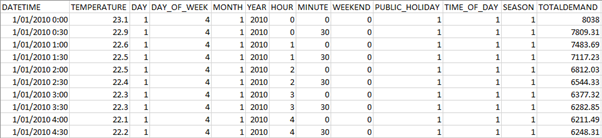
\includegraphics{first_10_records.png}
\caption{The first 10 records in the transformed dataset used for modelling of the neural networks.}\label{3.1}
\end{figure}

\hypertarget{assumptions}{%
\section{Assumptions}\label{assumptions}}

It is assumed that the provided data was accurate and that the actual
demand figures are correct. There may be errors in temperature
recordings as evident by missing records for temperature. In addition to
that, recorded temperatures at one location may not be a true
representation for the entire region.

\bigskip

It is recognised that the Solar PV data influences the actual
electricity demand. Furthermore, it is assumed that currently there is
no mechanism to get this data to the granule of the region for each
timestamp.

\bigskip

With these limitations, the assumption is that it the given data is
sufficient to predict the forecast demand within a range 5-10\% of the
actual demand.

\bigskip

\hypertarget{modelling-methods}{%
\section{Modelling Methods}\label{modelling-methods}}

Before the dataset described in Chapter 3.3 could be used for modelling,
transformations were required for some attributes. Columns with ordinal
number values, including the columns DAY, DAY\_OF\_WEEK, MONTH, HOUR,
TIME\_OF\_DAY and SEASON, were transformed using one-hot encoding. The
dataset was then split into a training and test set. A minimum maximum
scalar was then fitted for each of continuous values in the training
set. This was performed on the TEMPERATURE and TOTALDEMAND columns where
values were proportionally reassigned to values between 0 and 1. These
fittings were then used to transform the TEMPERATURE and TOTALDEMAND
columns in both the training and test set. From experimentation we
limited the inputs to month and hour as categorical variables,
identifying whether it is a weekday or weekend and identifying if the
day was a public holiday.

\bigskip

The LSTM model has been designed to use the attributes of a designated
number of immediately previous timestamps to the record that is either
being trained or predicted. This number is set by a variable called
`time\_steps'. A function was then created to transform both the X value
for the training and test datasets into a three-dimensional matrix. The
three dimensions represent the number of records in the dataset, the
number of immediately prior records (time\_steps) to the current record
and the number of features used for these prior records. This therefore
means that for each dataset the first number of records, equal to the
value of the time\_steps variable, cannot be trained or predicted by the
model. This is because the number of previous records in the dataset for
these records is less than the value of the time\_steps variable. It
should also be noted that the total demand values from the previous
records were also included in the matrix of X values. The y value fed to
the neural network is the total demand for the current record being
either trained or predicted.

\bigskip

The neural network consists of a single layer bidirectional LSTM with 50
neurons which uses `relu' for the activation function. This feeds into a
single dense neuron. As part of the python tensorflow library, keras was
used to compile the model. Mean square error was used to measure the
performance of the model and Adam was used to optimise the model. When
fitting the model, 30 epochs were used with a batch size of 32 with 0.1
(10\%) of the training dataset set aside for validation. The values of
the test dataset were then used to make predictions for the y values of
the test dataset with an inverse transform then applied to restore these
predictions back to the pre-scaled values. Root Mean Square Error (RMSE)
was also used to determine how well the model was performing.

\bigskip

The test result was recorded along with the `DATETIME' timestamp,
temperature, actual and predicted demand in a .csv file for further
analysis and visualisation by any appropriate tools such as Tableau.

\bigskip

The built model and the scalers of temperature and demand were saved so
that the prediction program can work independently by loading this model
and scalers. Various combinations of the attributes were used until the
best combination was determined. The final columns used in the model
were TEMPERATURE, WEEKEND, PUBLIC\_HOLIDAY, MONTH (one-hot encoded),
HOUR(one-hot encoded) and TOTALDEMAND.

\bigskip

\hypertarget{prediction-algorithm}{%
\section{Prediction Algorithm}\label{prediction-algorithm}}

Based on the model, the forecast temperature is an important factor for
forecasting demand. The data for `time\_steps' (e.g., 24) number of
records of actual demand prior to the forecast period is also required
for the time series LSTM model to work. All other inputs can be prepared
based on the `DATETIME' timestamp.

\bigskip

Suppose the actual demand information available weekly is on Sunday
midday, and the requirement is to provide a forecast of demand for the
following week. With the forecast of temperature for that week, the
input data will be built with the appropriate timeslot related input,
temperature, with the actual demand field set to zero.

\bigskip

The last 24 timeslots of complete data records including actual demand
will be joined in front of the forecast records. The prediction program
loads the saved neural network model, the scalers for temperature and
demand and then loads the entire dataset and converts it to the
appropriate input format with the necessary scaling. As the month and
hour data (if the forecast is only for a few hours and not for 24 hours
or a week) will be limited, it can not use standard one hot encoding.
So, the program builds this encoding programmatically.

\bigskip

Once the input is transformed, the algorithm picks the first 24 records,
and predicts the demand for the 25th slot. While recording this
information for output, the actual demand for the 25th record will be
updated with this predicted demand value and the oldest record (1st
record) will be dropped.

\bigskip

Now having complete records for the first 24 records again, the above
process is repeated until all the necessary forecast demands having been
performed. Practically the future forecast demand is based on the
forecast, so it is possible to have the error build cumulatively.
However, if the actual demand data is available say every hour, then the
program can predict the forecast hourly with much accurate input. The
forecast period also will be decided by the stakeholders.

\bigskip

The test result was recorded along with the `DATETIME' time stamp,
temperature, predicted demand in a .csv file for distribution to
relevant stakeholders. The model can be re-trained every month or even
daily to cover latest environmental and policy impacts as training will
take less than 10 minutes on an average computer without the GPU support
for 3 year data.

\hypertarget{exploratory-data-analysis}{%
\chapter{Exploratory Data Analysis}\label{exploratory-data-analysis}}

\hypertarget{using-tableau}{%
\section{Using Tableau}\label{using-tableau}}

\textbf{Year to year monthly temperature-demand trend} \newline \newline
- Given temperature and demand data is from Jan'10 to Mar'21 \newline -
Monthly avg. temperature varies 2/3 degrees \newline - Demand is
comparatively higher during winter season (Jun-Aug) \newline - Overall
demand shows reduction in the recent years \newline

\begin{figure}[H]
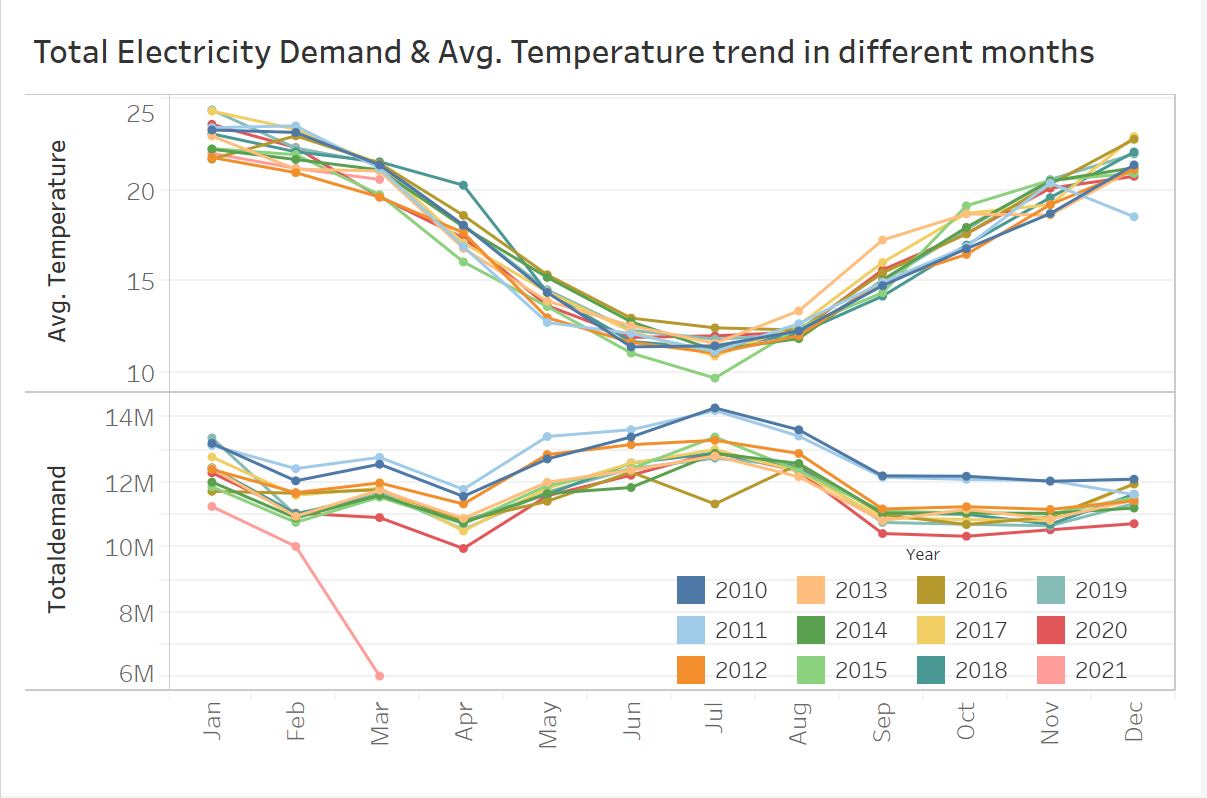
\includegraphics{snapshots1/Slide 2 snapshot.png}
\caption{Total Electricity Demand and Avg. Temperature trend in different months}\label{4.1}
\end{figure}

\textbf{Monthly temperature-demand in diff. weekdays trend} \newline
\newline - Different months have different demand pattern in different
weeks days \newline - Year to year the pattern is not same \newline

\begin{figure}[H]
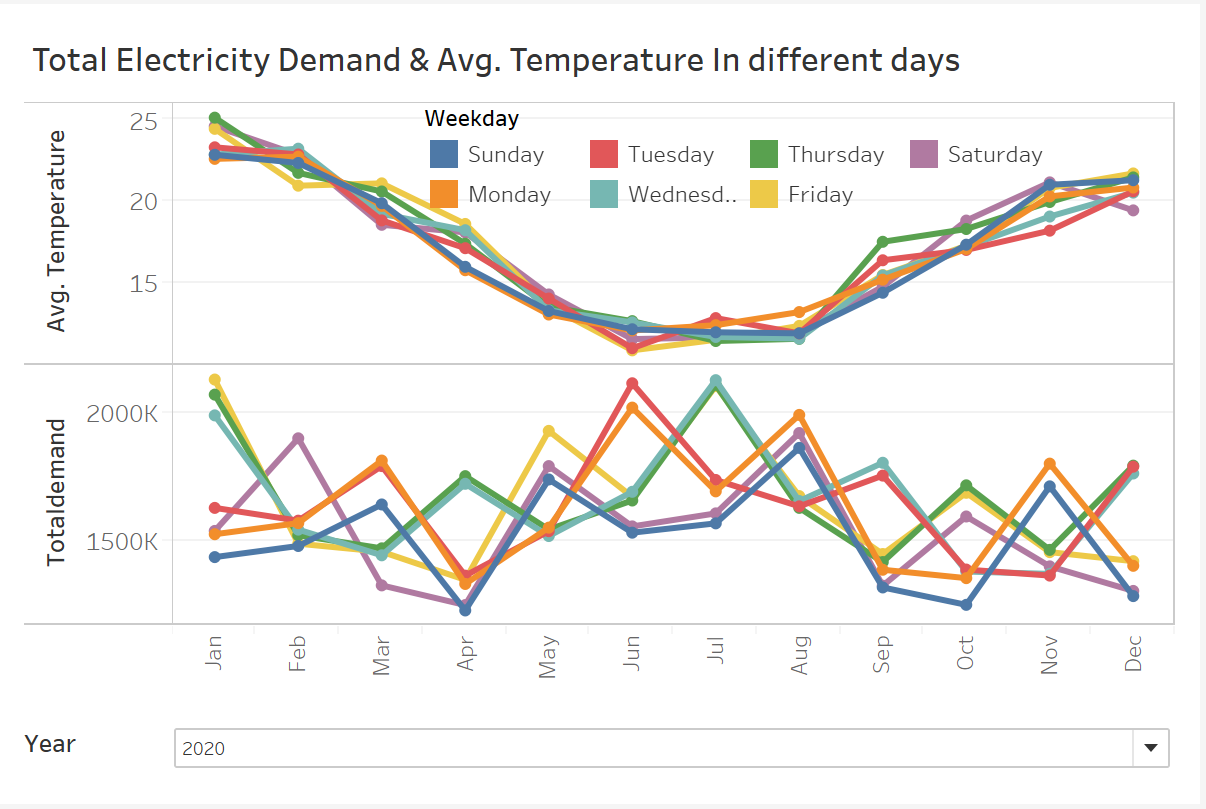
\includegraphics{snapshots1/Slide 3 snapshot 1.png}
\caption{Total Electricity Demand and Avg. Temperature trend in different days}\label{4.2}
\end{figure}

\begin{figure}[H]
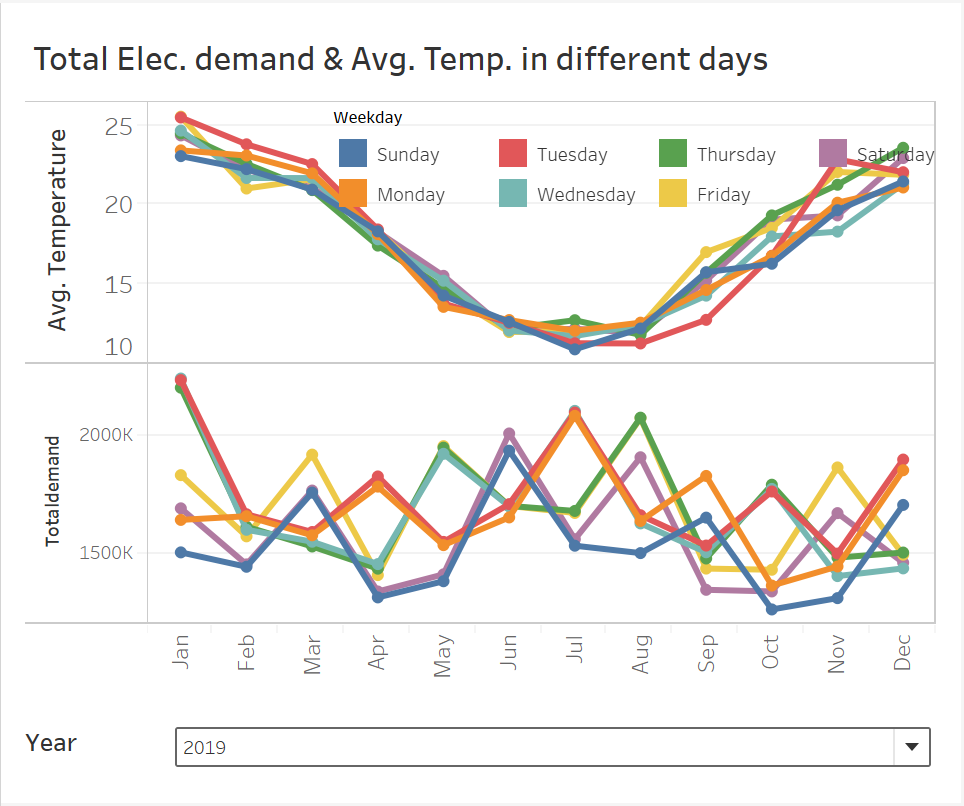
\includegraphics{snapshots1/Slide 3 snapshot 2.png}
\caption{Total Electricity Demand and Avg. Temperature trend in different days}\label{4.3}
\end{figure}

\textbf{Hourly temperature-demand in diff. weekdays trend} \newline
\newline - Demand somewhat follows temperature during off peak
(night-time) time \newline - Demand variation during daytime varies in
different days and not always proportional to temperature \newline

\begin{figure}[H]
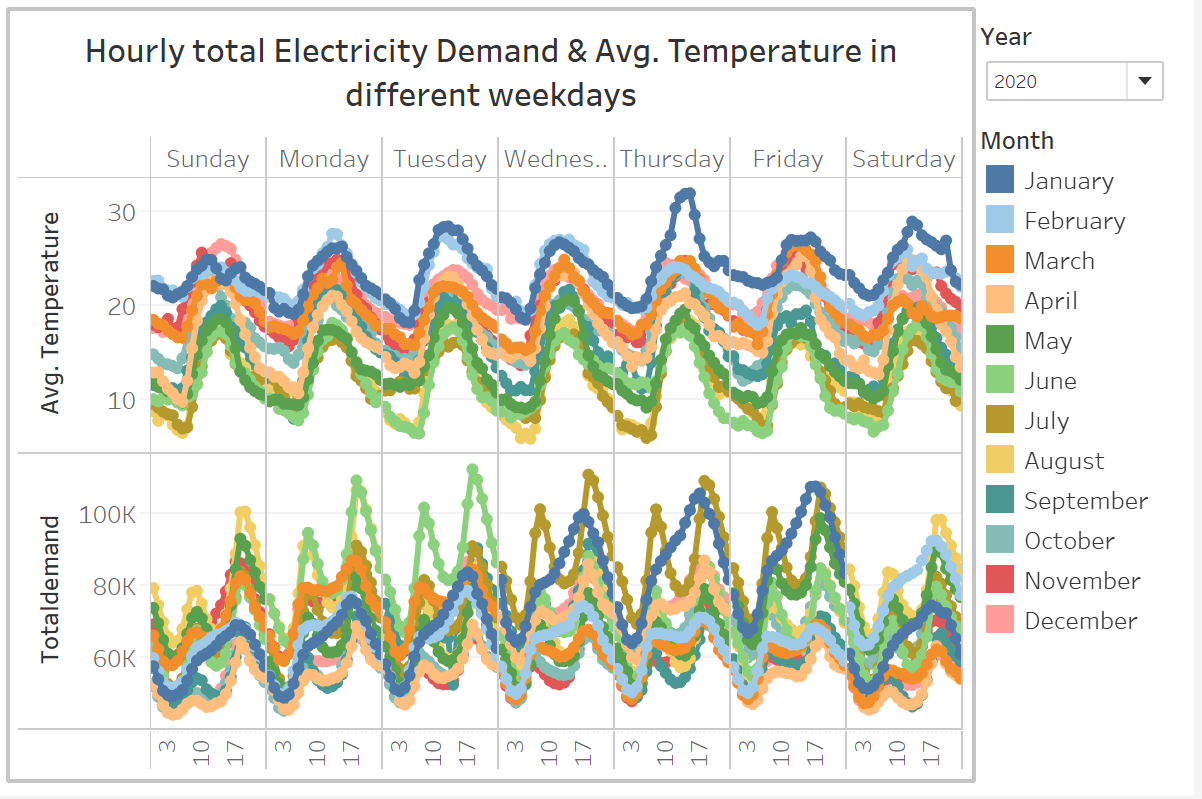
\includegraphics{snapshots1/Slide 4 snapshot 1.png}
\caption{Hourly total Electricity Demand and Avg. Temperature in different weekdays}\label{4.4}
\end{figure}

\begin{figure}[H]
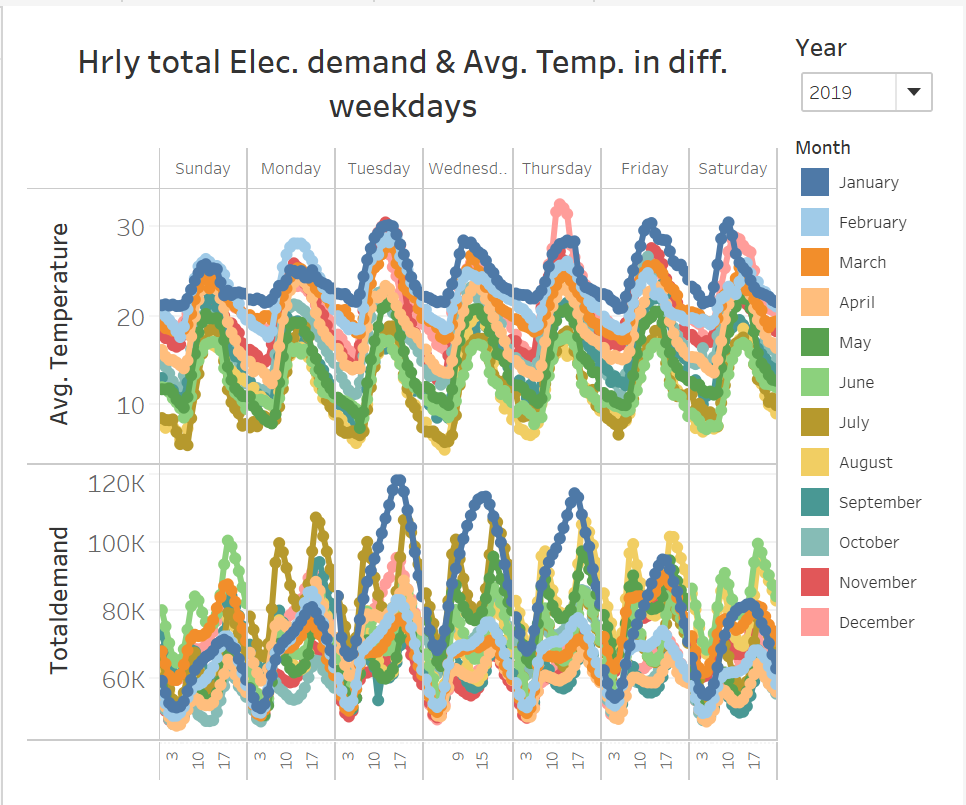
\includegraphics{snapshots1/Slide 4 snapshot 2.png}
\caption{Hourly total Electricity Demand and Avg. Temperature in different weekdays}\label{4.5}
\end{figure}

\textbf{Hourly Forecast vs.~Demand (Jan and Aug 2020 first 10 days)}
\newline \newline - Current forecasts are pretty good in some hours and
in some months \newline - Forecast suffers accuracy during daytime
\newline

\begin{figure}[H]
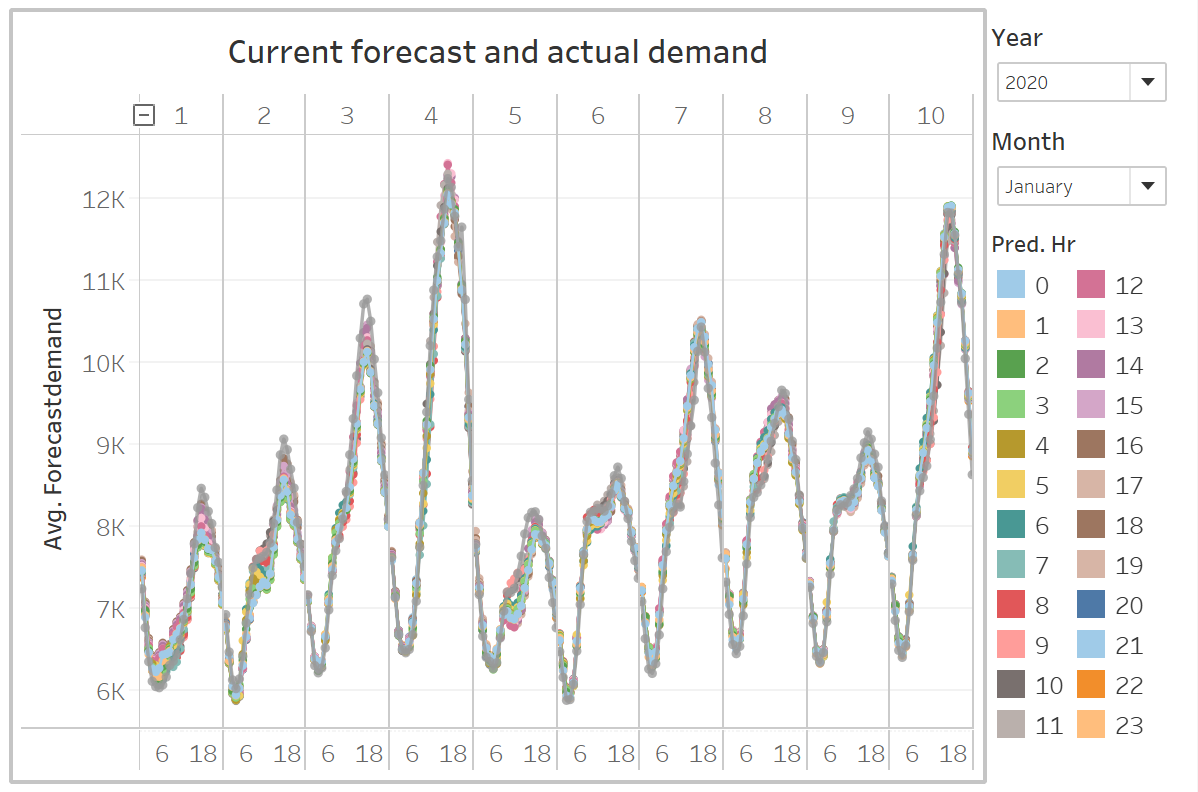
\includegraphics{snapshots1/Slide 5 snapshot 1.png}
\caption{Current forecast and actual demand}\label{4.6}
\end{figure}

\begin{figure}[H]
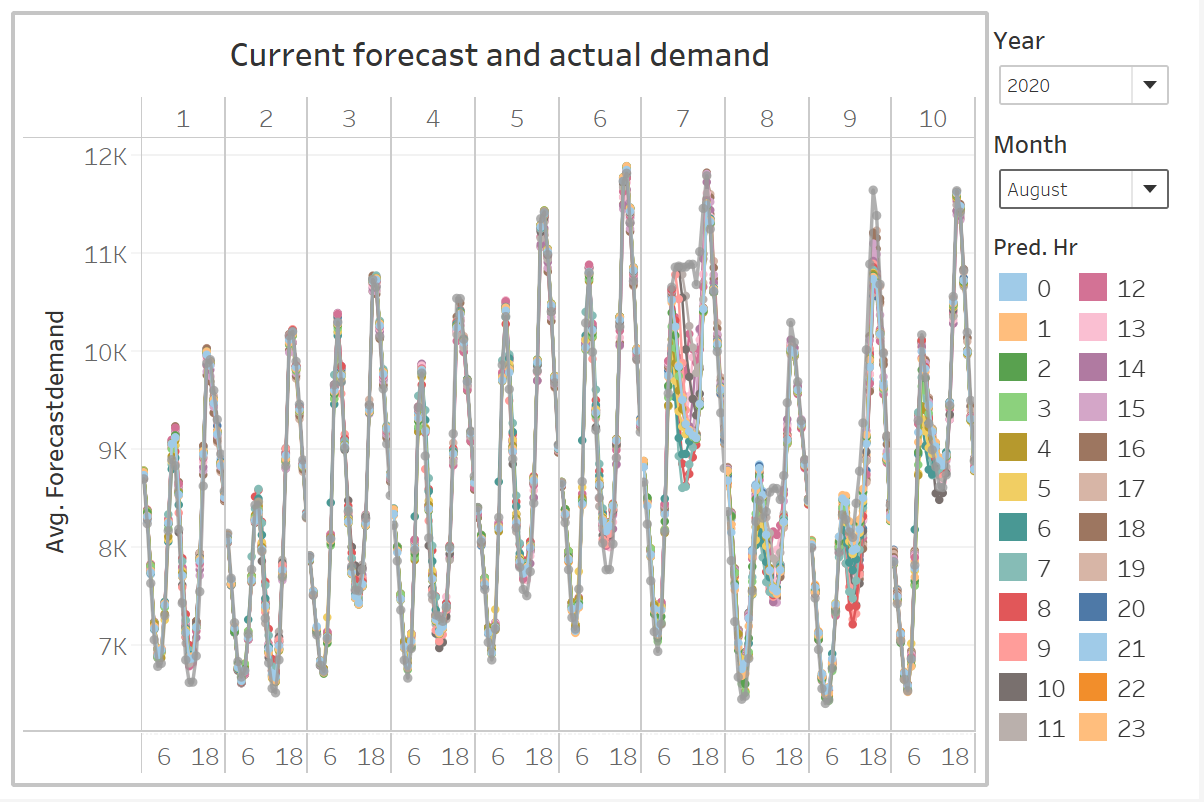
\includegraphics{snapshots1/Slide 5 snapshot 2.png}
\caption{Current forecast and actual demand}\label{4.7}
\end{figure}

\textbf{2021 prediction results vs actual demand} \newline \newline -
LSTM model output shows good performance during off peak time \newline -
In some month (March) prediction seems very good

\begin{figure}[H]
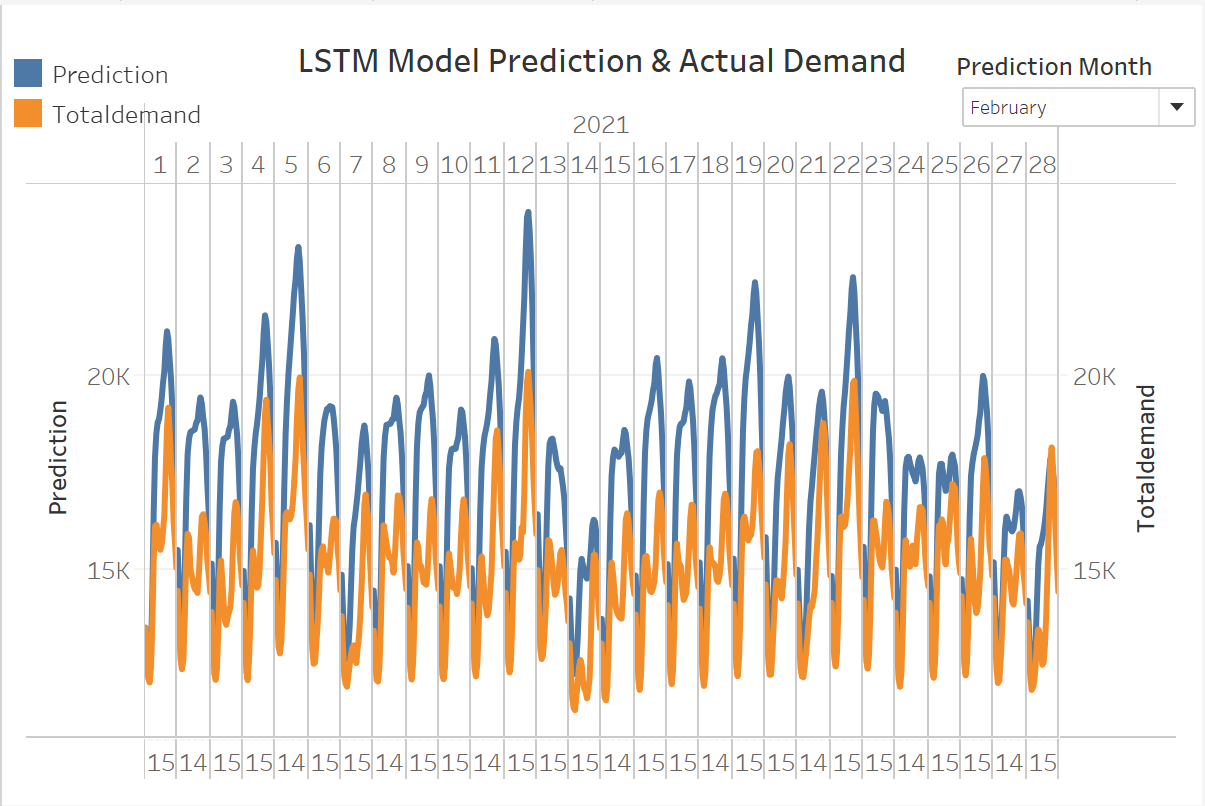
\includegraphics{snapshots1/Slide 6 snapshot 1.png}
\caption{LSTM Model Prediction and Actual Demand}\label{4.8}
\end{figure}

\begin{figure}[H]
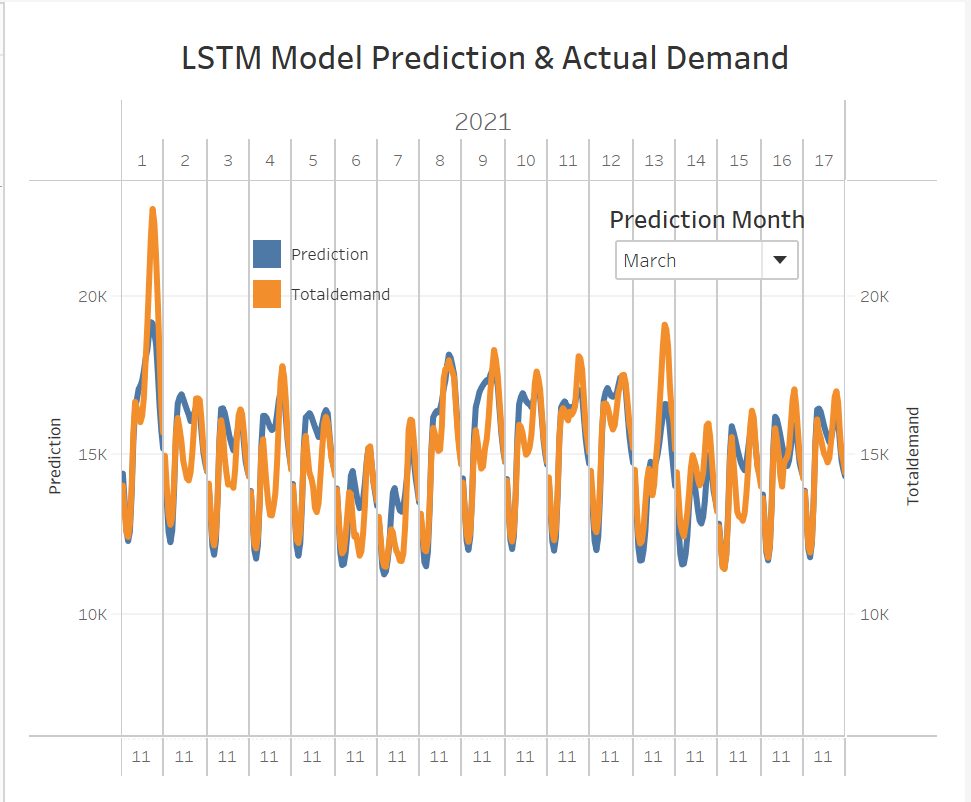
\includegraphics{snapshots1/Slide 6 snapshot 2.png}
\caption{LSTM Model Prediction and Actual Demand}\label{4.9}
\end{figure}

\hypertarget{analysis-and-results}{%
\chapter{Analysis and Results}\label{analysis-and-results}}

\hypertarget{a-first-model}{%
\section{A First Model}\label{a-first-model}}

The categorical variables: month, day of the week and the 48 half-hour
timestamps along with the temperature and actual demand were used to
train the Multilayer Perceptron (MLP) model. With various tunings of
hyper parameters with regards to dropout, learning rate, hidden layers
and neurons, the best achieved Root Mean Square Error (RMSE) was about
450-500MW on both the train and test dataset. Based on this result, it
was clearly indicating that the bias is high in the morning session
timestamps, which could suggest that some features were missing and that
the model didn't incorporate all of the variation in energy demand. One
of these key missing features here is Solar PV, which is unable to be
accurately provided for each region and timeslot at this stage.

\bigskip

The MLP model used 3 hidden layers of 200, 100 and 200 neurons with the
final output layer, all using `Relu' as the activation function. The
ultimate model should be significantly better than the error associated
with this MLP model, and the benchmark RMSE should be around 85MW as per
the currently deployed model. The provided data is a time series which
should hence produce a better result. Based on the literature review, a
LSTM structure is the ideal model to work with.

\bigskip

\hypertarget{lstm-model-only-using-previous-total-demand-values}{%
\section{LSTM Model -- Only Using Previous Total Demand
Values}\label{lstm-model-only-using-previous-total-demand-values}}

The early LSTM structure, which happens to be a mono-directional model
just uses the time series of actual demand with a lookback of 24
records, produced a significantly better result than the first model.
The model trained with an RMSE of 100MW, which was superior to the
450-500MW RMSE achieved previously. Naturally, this model was picked for
fine-tuning with appropriate feature inputs and hyper parameters.

\bigskip

\hypertarget{ulimate-lstm-model}{%
\section{Ulimate LSTM Model}\label{ulimate-lstm-model}}

The temperature is a key feature in the dataset - extreme temperatures
require heavy cooling or heating (depending on where they are on the
spectrum) which puts severe demand on electricity. Based on the time of
day, as well as if it is a weekday or weekend, the electricity usage
will differ. This implies various categorical inputs based on the
timestamp play a bigger role. As described in the modelling methods
chapter of the analysis, categorical variables span MONTH and HOUR along
with weekday/weekend status and whether it is a public holiday or not.
It was noted that the temperature and demand scaled between 0 and 1
which improved the result. A BIDRIECTIONAL LSTM structure takes a bit
more time to train but further improved the result.

\bigskip

The final model was produced with a 50 node bidirectional single LSTM
with `Relu' as activation function. This was trained with data from
2018-2020 with 30 epochs, a batch size of 32 and a lookback of 24
timestamps. Furthermore, a validation split of 10\% and test set of 2021
produced an excellent result, with an RMSE less than 70MW (66.55MW) on
test data as well as an average percentage difference of 0.66\%.

\hypertarget{discussion}{%
\chapter{Discussion}\label{discussion}}

The results presented in the previous chapter demonstrate that a
bidirectional LSTM presents an effective approach to developing accurate
forecasting models for energy demand. The bidirectional LSTM outperforms
all other tested models, including a mono-directional LSTM and basic
MLP, which do not appear to have the same forecasting abilities in this
application with the time-series data with a limited amount of features.

\bigskip

The basic MLP model produced a mean square error of around 7 times
higher than the final model, which perhaps speaks of its inability to
work with this type of demand timeseries data. Part of this poor
performance is the difference in how inputs were processed for the
models - with the MLP treating each timestamp as a categorical variable.
In the final LSTM model, the timestamps are treated as a sequence which
may perhaps explain this reduction in error. It was also of note that
the morning timestamps often had the biggest errors associated with them
in the MLP model. Although it is difficult to theorise the variation
here, a possible explanation for poor performance in the MLP model in
this specific area is that energy demand dramatically picks up once
people start to wake up and that the categories associated with the
early morning timestamps have miscalculated weights in the network.

\bigskip

The LSTM model that was originally tested overcame this issue of
treating the timestamps as categories - rather it took the timestamps in
sequence which appeared to dramatically decrease the RMSE, approaching
those benchmark error figures of 85MW. Most of the variation in energy
demand was captured here and no consistent trends were found in the
errors unlike in the MLP model. As was discovered in the literature
review prior to the analysis, this was expected as LSTM networks are
highly suited for classification and regression prediction problems,
based on time series data - which this energy demand dataset is.

\bigskip

The final bidirectional model was far superior to all models tested,
beats benchmark RMSE figures and gives sufficient evidence to the client
that this can be used profitably to price energy. Due to the model being
market-leading, it can both be used for a variety of reasons including
for private investors, market efficiency or to aide governments in
appropriate electricity distribution. The model works on the basis of
fairly straightforward idea when compared to the mono-directional LSTM.
The main difference here is that the first recurrent layer in the
network is duplicated so that there are two layers alongside each other.
Furthermore, the first layer receives the input sequence as an input
as-is, whilst the second layer is provided a reversed copy of the input
sequence.

\bigskip

As mentioned previously, perhaps the addition of extra datasets (either
Solar PV data or otherwise) with timestamps associated may improve the
quality of predictions and reduce the model error even further. Although
the bidirectional LSTM worked extremely well for this application, other
network architectures may also be explored in future.

\hypertarget{conclusion-and-further-issues}{%
\chapter{Conclusion and Further
Issues}\label{conclusion-and-further-issues}}

The bi-directional Long short-term memory (LSTM) model performs well
when predicting electricity demand for NSW, Australia. Using the last 24
timestamps, the pre-processed data is given as input which is then fed
through the model and gives a Root Mean Square Error (RMSE) of 66.55MW
and an average percentage error difference of 0.66\% in the sample
tested. This can be used profitably by the client through the
appropriate pricing based on model outputs, with an appropriate profit
margin to account for variance in the model. Although the bi-directional
LSTM has worked well, there is no doubt that more data (i.e.~Solar PV
data or even an increased granularity in timestamps) could decrease the
model error and make pricing more efficient for the client. Furthermore,
other deep-learning architectures may be explored as well in the future,
even though this model architecture worked successfully on this
occasion. However, it is important to note, as was evident in this
analysis, that inducing a more complex network structure to model the
data does not always improve model accuracy.

\bibliographystyle{elsarticle-num}
\bibliography{references}

\hypertarget{appendix}{%
\chapter*{Appendix}\label{appendix}}
\addcontentsline{toc}{chapter}{Appendix}

\hypertarget{codes}{%
\section*{\texorpdfstring{\textbf{Codes}}{Codes}}\label{codes}}
\addcontentsline{toc}{section}{\textbf{Codes}}

\begin{figure}[H]
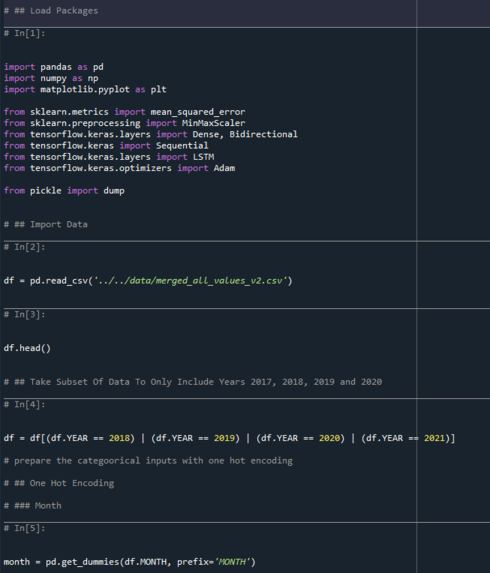
\includegraphics{snapshots1/LSTM_Build_Model_1.png}
\caption{LSTM Model Build 1}\label{ModelBuild1}
\end{figure}

\begin{figure}[H]
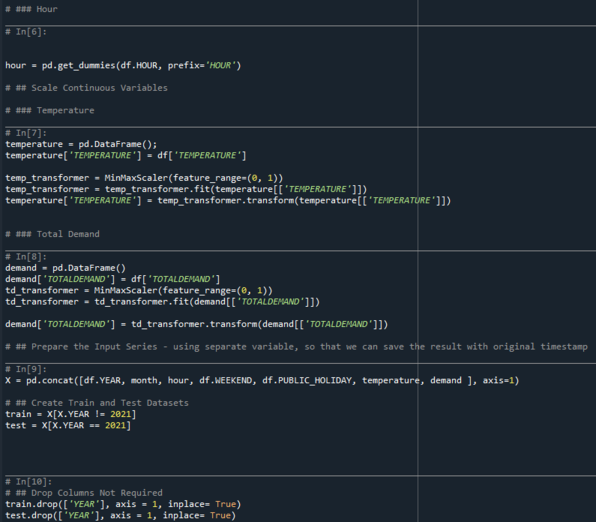
\includegraphics{snapshots1/LSTM_Build_Model_2.png}
\caption{LSTM Model Build 2}\label{ModelBuild2}
\end{figure}

\begin{figure}[H]
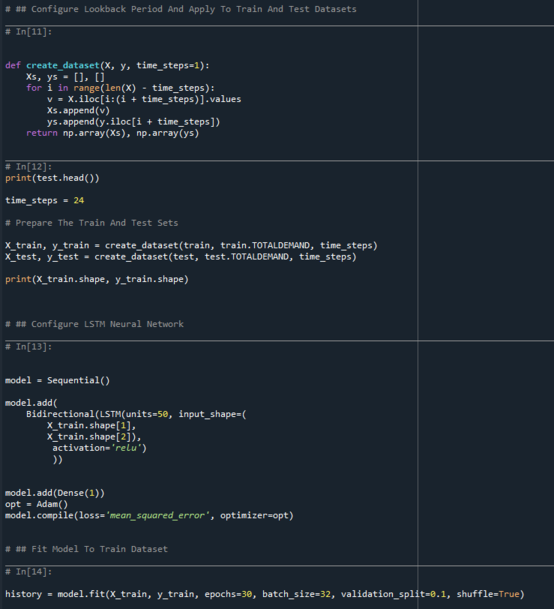
\includegraphics{snapshots1/LSTM_Build_Model_3.png}
\caption{LSTM Model Build 3}\label{ModelBuild3}
\end{figure}

\begin{figure}[H]
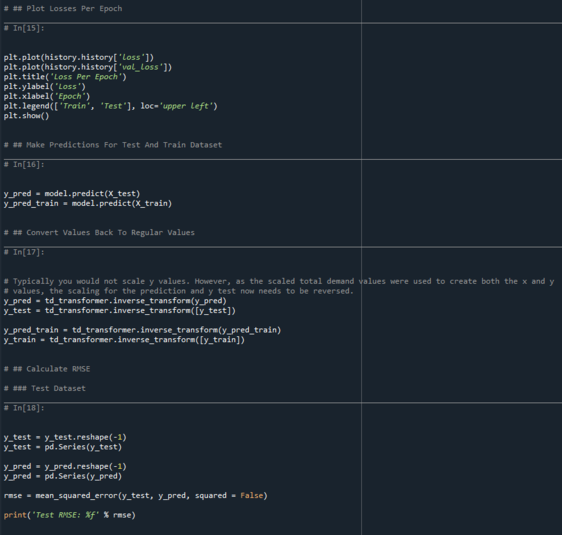
\includegraphics{snapshots1/LSTM_Build_Model_4.png}
\caption{LSTM Model Build 4}\label{ModelBuild4}
\end{figure}

\begin{figure}[H]
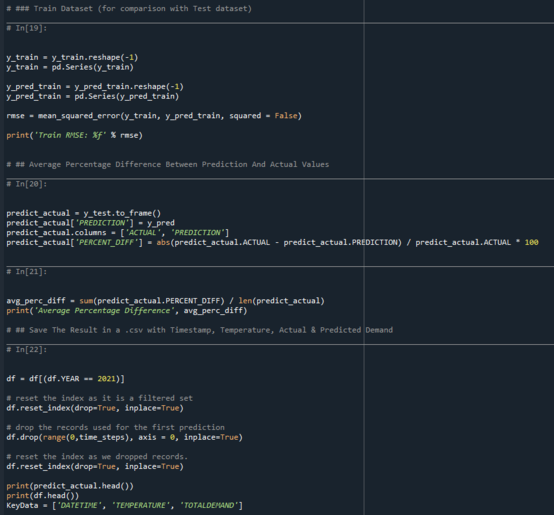
\includegraphics{snapshots1/LSTM_Build_Model_5.png}
\caption{LSTM Model Build 5}\label{ModelBuild5}
\end{figure}

\begin{figure}[H]
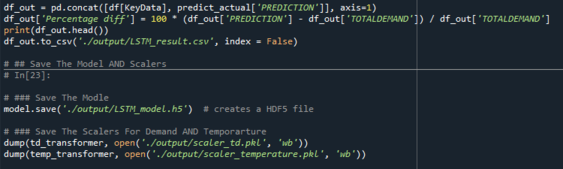
\includegraphics{snapshots1/LSTM_Build_Model_6.png}
\caption{LSTM Model Build 6}\label{ModelBuild6}
\end{figure}

\begin{figure}[H]
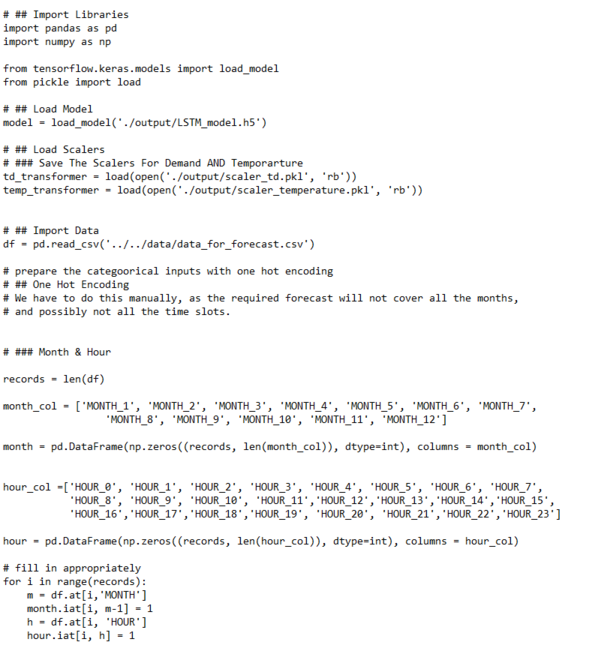
\includegraphics{snapshots1/new LSTM_Forecast_1.png}
\caption{LSTM Forecast 1}\label{LSTMForecast1}
\end{figure}

\begin{figure}[H]
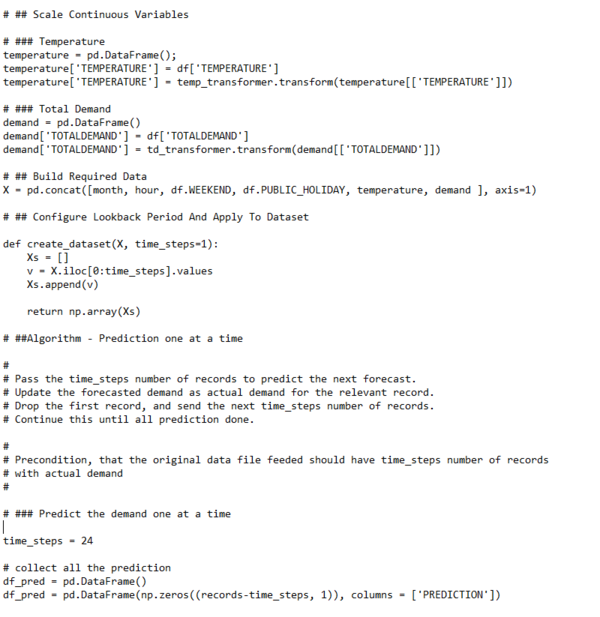
\includegraphics{snapshots1/new LSTM_Forecast_2.png}
\caption{LSTM Forecast 2}\label{LSTMForecast2}
\end{figure}

\begin{figure}[H]
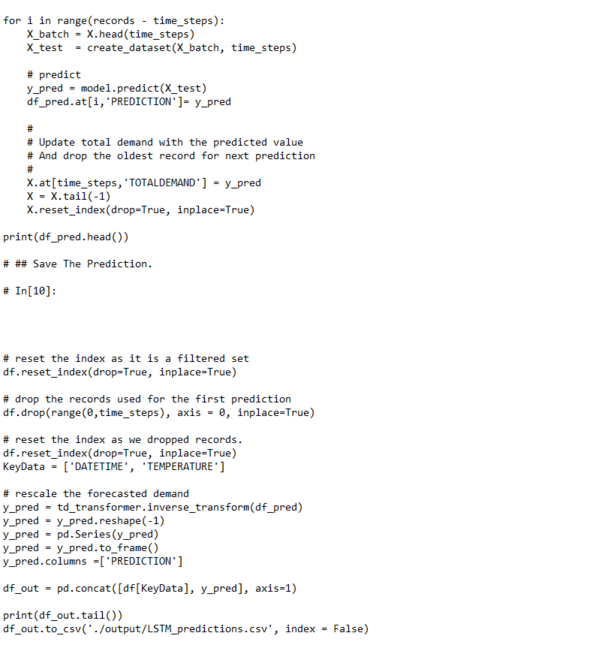
\includegraphics{snapshots1/new LSTM_Forecast_3.png}
\caption{LSTM Forecast 3}\label{LSTMForecast3}
\end{figure}

\hypertarget{model-results}{%
\section*{\texorpdfstring{\textbf{Model
Results}}{Model Results}}\label{model-results}}
\addcontentsline{toc}{section}{\textbf{Model Results}}

\begin{figure}[H]
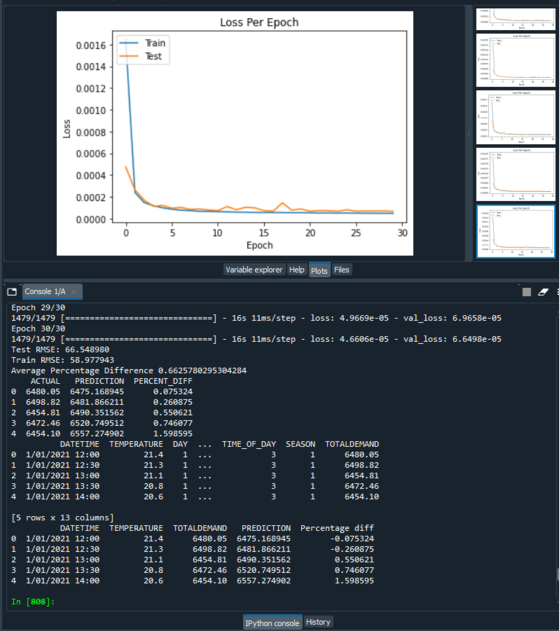
\includegraphics{snapshots1/LSTM Test Result 1.png}
\caption{LSTM Model Test Result}\label{ModelResult}
\end{figure}







\end{document}

